%!TEX TS-program = xelatex
%!TEX encoding = UTF-8 Unicode
\documentclass[12pt, xcolor=dvipsnames]{beamer}
\definecolor{slight}{gray}{0.9}
\fboxsep=10pt
\usecolortheme[named=Royal Blue]{structure}
\useinnertheme{circles}
\usepackage[no-math]{fontspec}
\usepackage{xltxtra, xunicode}
\usepackage[utf8]{inputenc}
%\usepackage[sc, osf]{mathpazo}
\usepackage[minionint, lf, mathtabular]{MinionPro}
\setmainfont[Mapping=tex-text]{Minion Web Pro}
\setsansfont[Mapping=tex-text]{Myriad Web Pro}
\setmonofont[Scale=MatchLowercase]{Source Code Pro}
\usefonttheme{professionalfonts}
%% 中文字配置
\usepackage[
CJKmath=true, indentfirst=false, PunctStyle={quanjiao},
CheckSingle=true, SlantFont, BoldFont
]{xeCJK}
\setCJKmainfont[Scale=0.9, BoldFont=Hiragino Mincho ProN W6]{Hiragino Mincho ProN W3}
%\setCJKmainfont[Scale=0.9, BoldFont=Noto Sans CJK JP Bold]{Noto Sans CJK JP Medium}
\setCJKsansfont[Scale=0.9, BoldFont=Hiragino Sans W6]{Hiragino Sans W4}
%\setCJKsansfont[Scale=0.9, BoldFont=Hiragino Sans CNS W6]{Hiragino Sans CNS W3}
%\setCJKsansfont[Scale=0.9, BoldFont=Hiragino Sans W7]{Hiragino Sans W4}
%\setCJKsansfont[Scale=0.9, BoldFont=Source Han Sans UI TC Bold]{Source Han Sans UI TC Regular}
%\setCJKsansfont[Scale=0.9, BoldFont=PingFang TC Semibold]{PingFang TC Regular}
\setCJKmonofont[Scale=0.9, BoldFont=Yuanti TC Regular]{Hiragino Maru Gothic ProN W4}
\usepackage{fancyvrb, attachfile2, pstricks}
\usepackage{graphicx}
\setbeamerfont{page number in head/foot}{size=\tiny}
\setbeamertemplate{footline}[frame number]
\usepackage{xmpmulti, booktabs, multicol}
\setbeamertemplate{navigation symbols}{}
\let\WriteBookmarks\relax
\usepackage{dcolumn}
\newcolumntype{.}[1]{D{.}{.}{#1}}
\newcolumntype{,}[1]{D{,}{,}{#1}}

\linespread{1.25}

\setbeamersize{text margin left=.8em, text margin right=.6em}

\makeatletter
\defbeamertemplate{itemize item}{mycircle}{\LARGE\raise-1.6pt\hbox{\textbullet}}
\makeatother

\setbeamertemplate{itemize item}[mycircle]
\setbeamertemplate{itemize subitem}[triangle]
\setlength\leftmargini{1.3em}
\setlength\leftmarginii{1em}


%\CTXFR
\title{\bf{\Huge {}\\[-2mm] Principles of Economics \\[2mm] Review Session}}
\author{{\Large 張耕齊\\[2mm] Keng-Chi Chang}}
\institute{{}\\[-7mm]\footnotesize\tt{<r03323070@ntu.edu.tw>}\\[2mm]}
\date{\large 2016.12.7}
\begin{document}
\fontsize{12}{14pt}\selectfont

\begin{frame}
\titlepage
\end{frame}





\begin{frame}
\frametitle{\bf §12.6 Price Discrimination 差別取價}
\begin{itemize}
\item Ways to restore some efficiency loss under monopoly?
\item First-degree: Charge the maximum willingness to pay for each customer
\begin{itemize}
\item This can fully restore social surplus, in an unequal way
\item Hard to achieve since you need to know many information
\item Ex. Panama Canal's pricing
\end{itemize}
\item Second-degree: Charge based on quantity of purchase
\begin{itemize}
\item Let those who has lower willingness to pay to self-select and buy at different quantity
\item Ex. Discount coupons, quantity discounts, 第二件六折
\end{itemize}
\item Third-degree: Charge based on characteristics of customers
\begin{itemize}
\item Some people may have lower willingness to pay, such as students
\item Ex. Student tickets, airline tickets, movie tickets
\end{itemize}
\end{itemize}
\end{frame}

\begin{frame}
\frametitle{\bf First-degree Price Discrimination}
\begin{center}
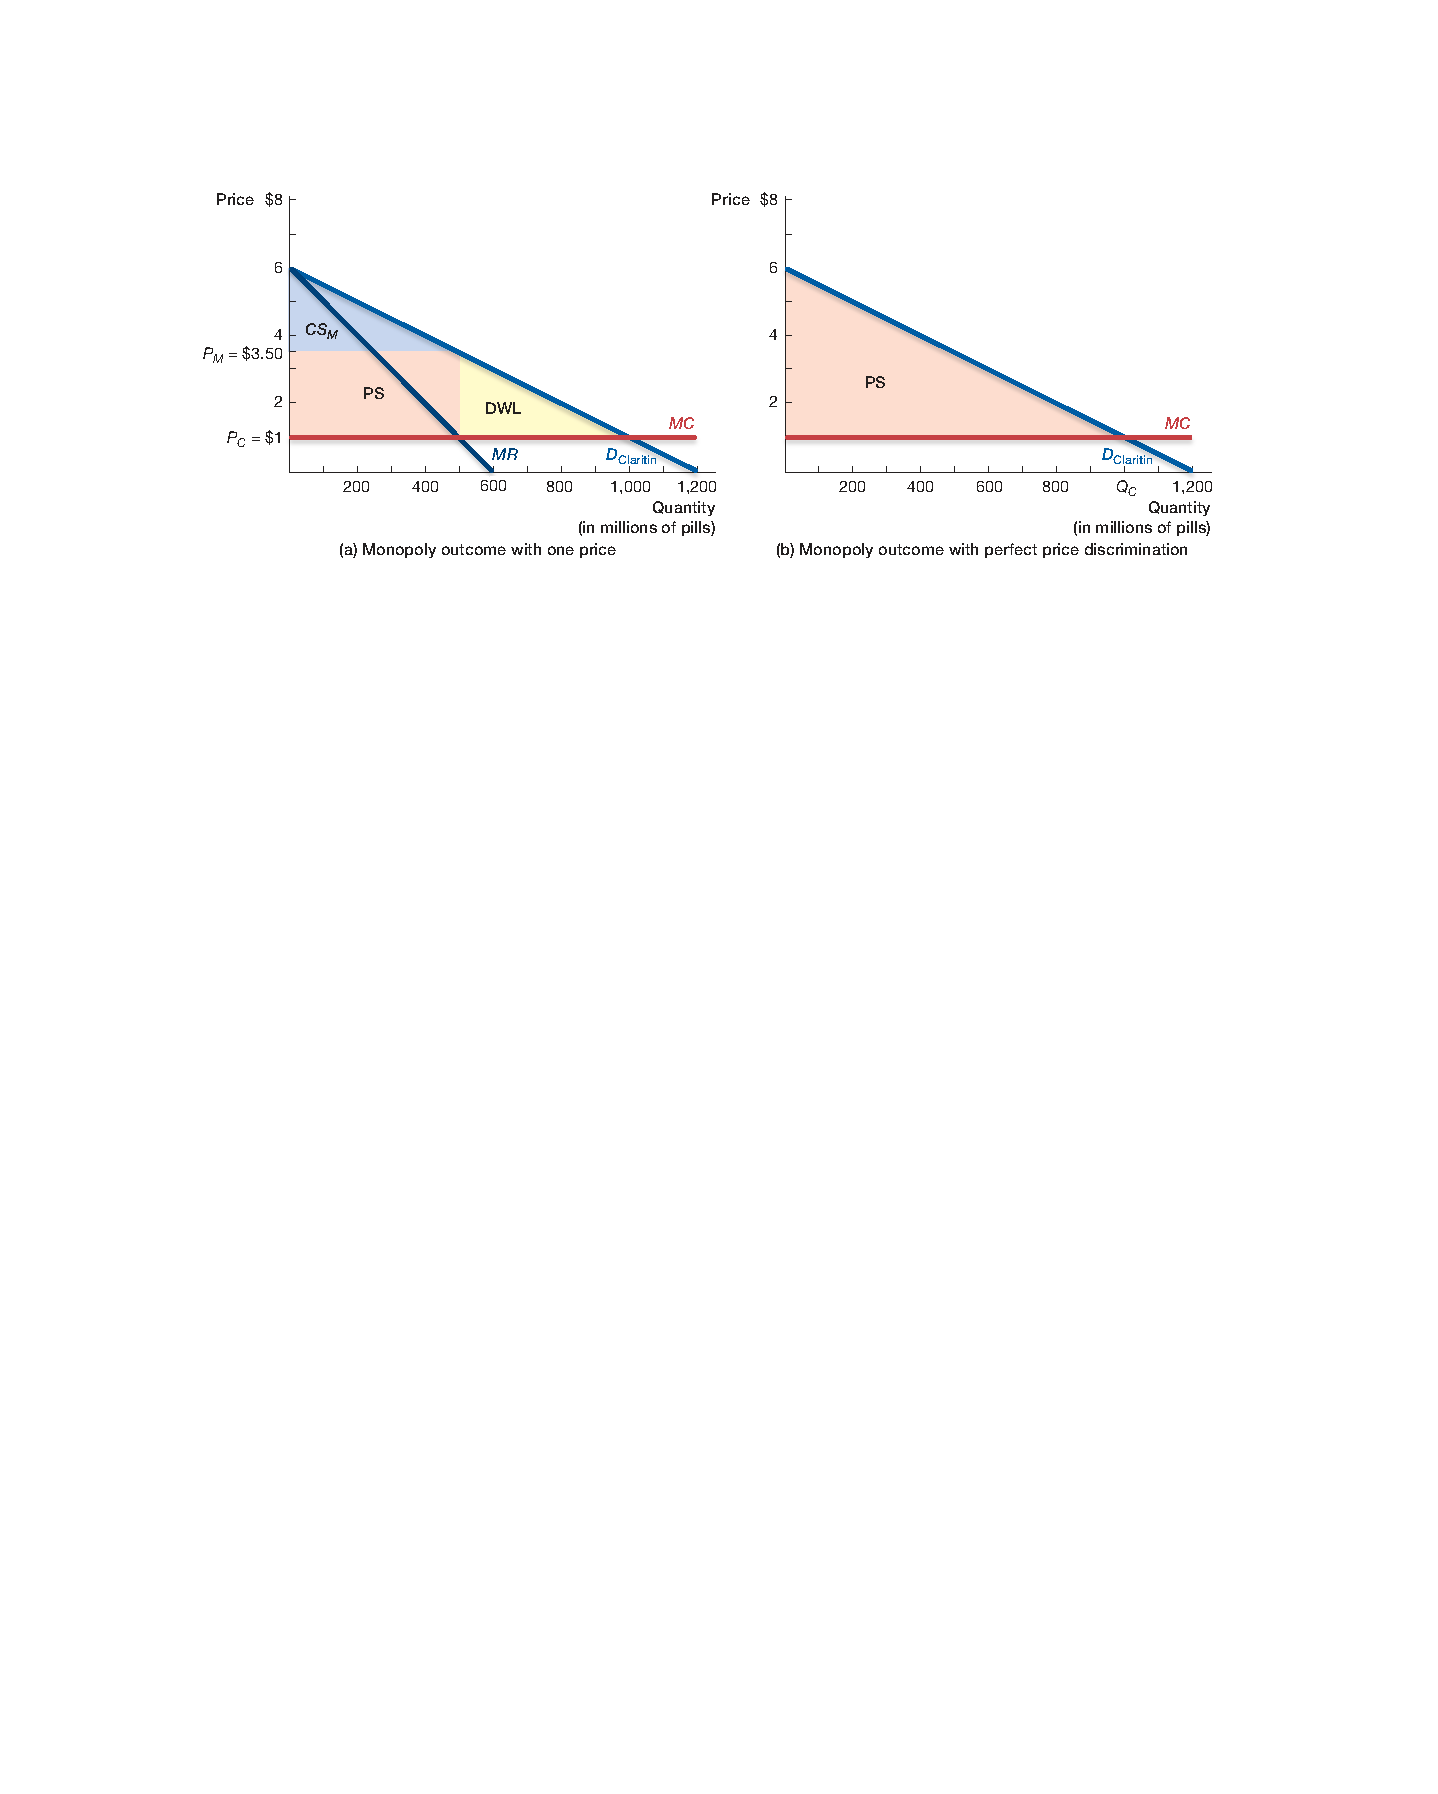
\includegraphics[width=\linewidth]{figures/13.pdf}
\end{center}
\end{frame}

\begin{frame}
\frametitle{\bf Monopolist's Profit}
\begin{center}
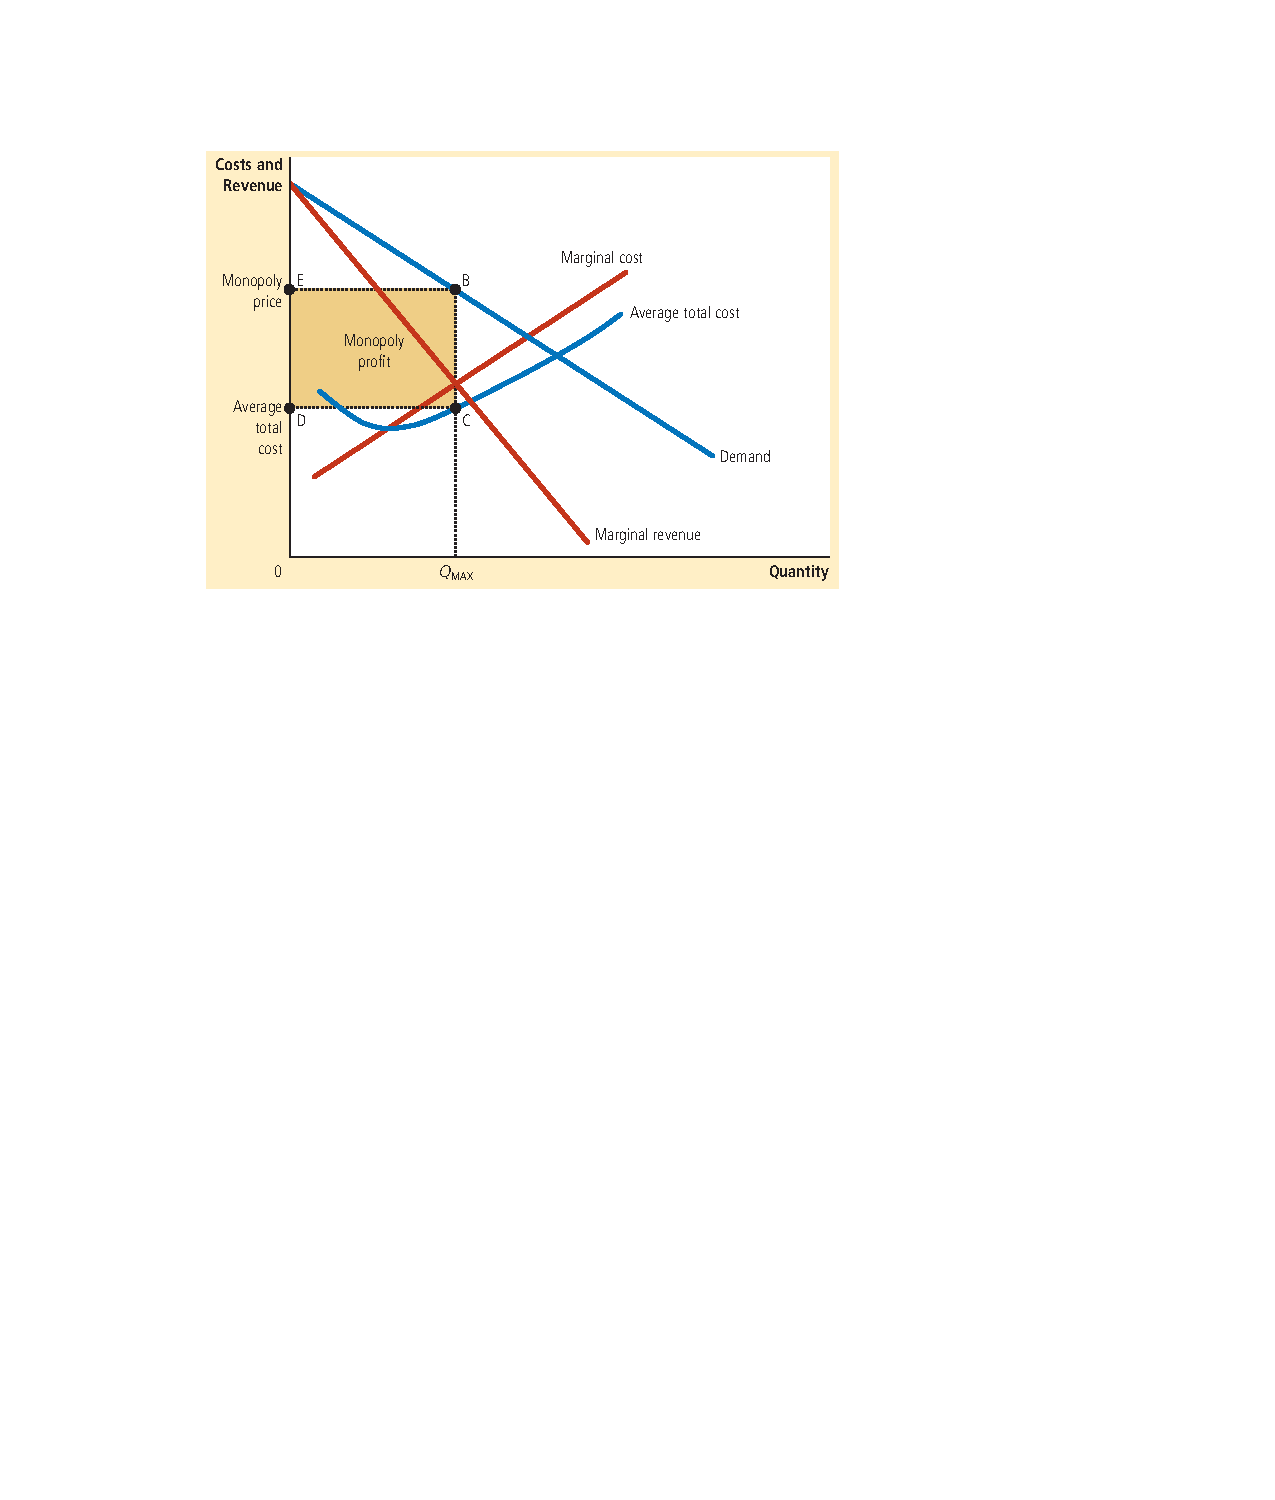
\includegraphics[width=.9\linewidth]{figures/profit.pdf}
\end{center}
\end{frame}




\begin{frame}
\small \textsf{\bfseries ALL 12-11.} Imagine that you arrive at an economics experiment with six other people and are told that you will simulate a market. You will be the only seller. The other five people will be assigned a dollar value that they will receive if they buy the good for any amount of money (so if a person's value is \$6, he will buy the good for any price less than \$6 and will be happy). You are also given the following demand curve and told that it represents the values that the ``buyers'' are assigned:
\begin{center}
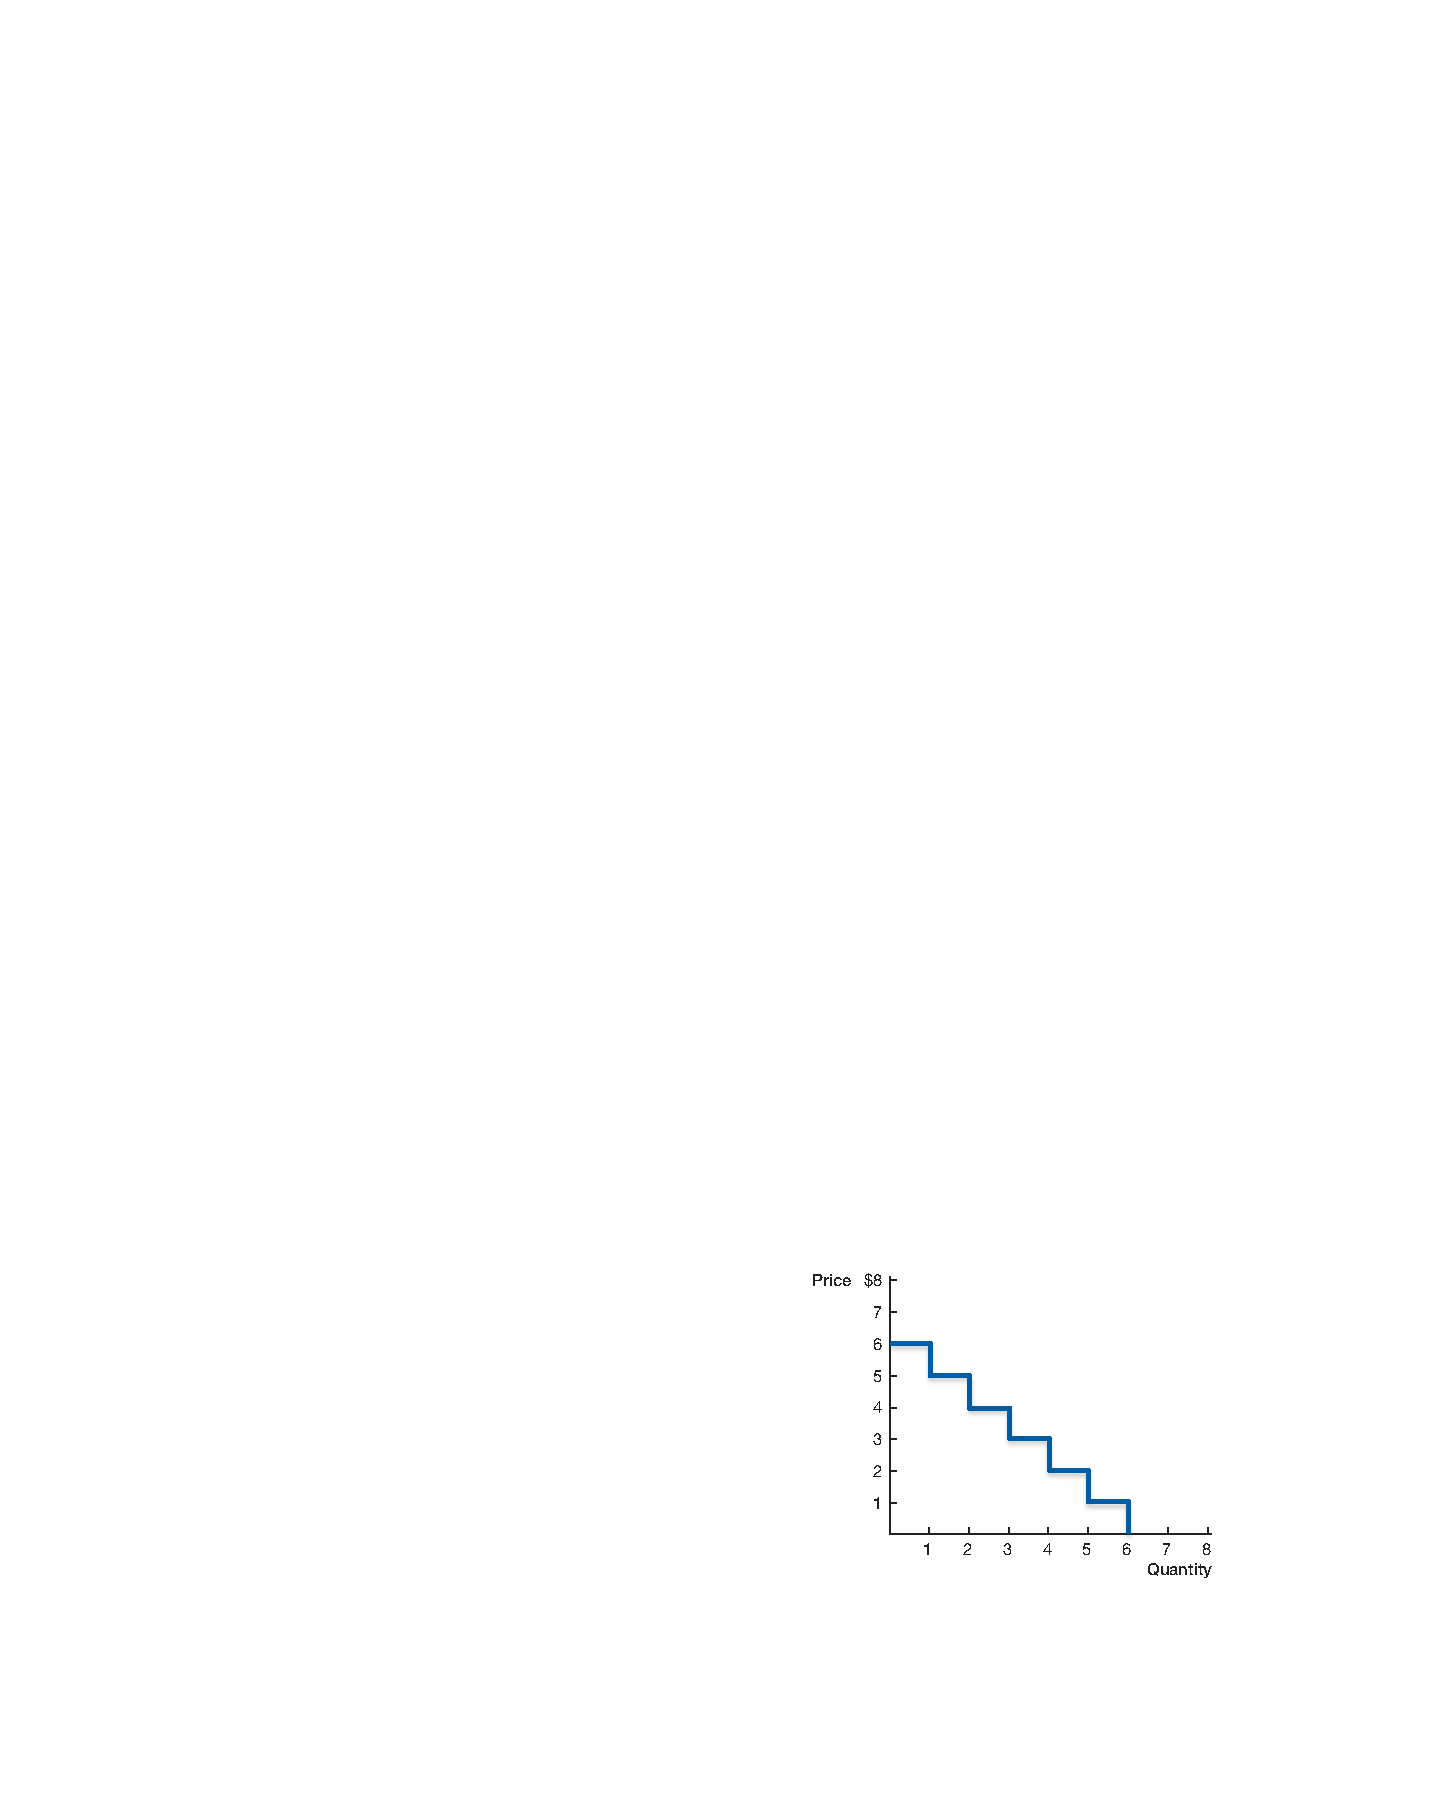
\includegraphics[width=.5\linewidth]{figures/p11.pdf}
\end{center}
\end{frame}


\begin{frame}
\small
\begin{enumerate}\itemsep-0.5ex 
\item[a.] If you are told that you can produce as many units as you like at a cost of \$2 per unit, what would your marginal cost curve look like? Add the marginal cost curve that you face as the monopolist to the graph.
\item[b.] Draw the marginal revenue curve that you face as the monopolist, based on the demand curve given above.
\item[c.] What price would you set and what quantity would you produce if you have to post one price at which everyone can purchase the good?
\item[d.] Based on the price and quantity you selected in part c, what would consumer surplus be? What would producer surplus be? Is there a deadweight loss?
\item[e.] Imagine that you are told that now you can have a discussion with each buyer privately to negotiate a price. Would you still charge everyone the same price? Explain your answer.
\item[f.] Calculate the surplus and the deadweight loss for the scenario with perfect price discrimination.
\end{enumerate}
\end{frame}


\begin{frame}
\textsf{\bfseries 2009 Multiple Choice Q5.} 
Price discrimination is a rational strategy for a profitmaximizing monopolist when
\begin{enumerate}\itemsep-0.5ex 
\item[A.] The monopolist finds itself able to produce only limited quantities of output.
\item[B.] Consumers are unable to be segmented into identifiable markets.
\item[C.] The monopolist wishes to increase the deadweight loss that results from profit maximizing behavior.
\item[D.] There is no opportunity for arbitrage across market segments.
\end{enumerate}
\end{frame}


\begin{frame}
\textsf{\bfseries 2015 True or False Q6.} 
If the customers of a monopolist could get together and bribe him to act like a competitor, then they could make both themselves and him better off.\\[4mm]
\textsf{\bfseries 2015 True or False Q7.} 
If Hewlett Packard could require all HP laser jet printer owners to buy all of their toner cartridges directly from HP, it would charge monopoly prices for those toner cartridges.\\[4mm]
\textsf{\bfseries 2015 True or False Q8.} 
A profit-maximizing monopolist whose firm was a source of negative externalities might produce exactly the socially optimal level of output. 
\end{frame}


\end{document}